\noindent
\begin{minipage}[t]{0.26\textwidth}
    \vspace{0pt}%
    % Hình 4
    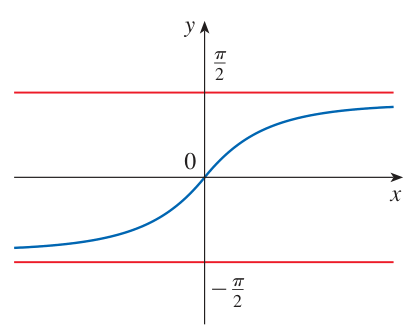
\includegraphics[width=\linewidth]{images/p0164_fig1.png}
    \vspace{2pt}
    
    {\small\textbf{\textsf{HÌNH 4}}}\\
    {\small $y = \tan^{-1}x$}
    
    \vspace{56pt}
    
    % Hình 5
    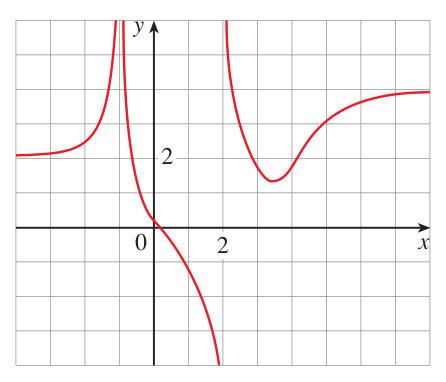
\includegraphics[width=\linewidth]{images/p0164_fig2.png}
    \vspace{2pt}
    
    {\small\textbf{\textsf{HÌNH 5}}}
    
    \vspace{130pt}
    
    % Hình 6
    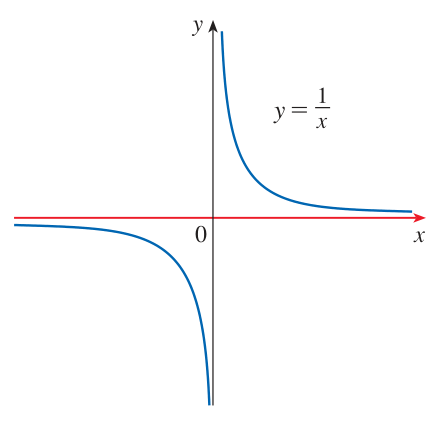
\includegraphics[width=\linewidth]{images/p0164_fig3.png}
    \vspace{2pt}
    
    {\small\textbf{\textsf{HÌNH 6}}}\\
    {\footnotesize $\displaystyle \lim_{x \to \infty} \frac{1}{x} = 0,\;\lim_{x \to -\infty} \frac{1}{x} = 0$}
\end{minipage}%
\hfill
\begin{minipage}[t]{0.71\textwidth}
    \vspace{0pt}%
    Chẳng hạn, đường cong được minh họa trong Hình 1 có đường thẳng $y = 1$ là một tiệm cận ngang vì
    \[
    \lim_{x \to \infty} \frac{x^2 - 1}{x^2 + 1} = 1
    \]
    Một ví dụ về đường cong có hai tiệm cận ngang là $y = \tan^{-1}x$. (Xem Hình 4.) Trên thực tế,
    
    \vspace{0.4em}
    \noindent
    \rlap{\tcbox[colback=white, colframe=stewartred, boxrule=0.8pt, arc=0mm, size=small, on line]{\bfseries\color{stewartred}\textsf{4}}}%
    \centering
    \tcbox[colback=white, colframe=stewartred, boxrule=0.8pt, arc=0mm, top=4.5pt, bottom=4.5pt, left=18pt, right=18pt]{%
        $\displaystyle \lim_{x \to -\infty} \tan^{-1}x = -\frac{\pi}{2}$%
        \qquad\qquad%
        $\displaystyle \lim_{x \to \infty} \tan^{-1}x = \frac{\pi}{2}$%
    }\par
    \vspace{0.4em}

    \noindent
    do đó cả hai đường thẳng $y = -\pi/2$ và $y = \pi/2$ đều là các tiệm cận ngang. (Điều này suy ra từ việc các đường thẳng $x = \pm\pi/2$ là các tiệm cận đứng của đồ thị hàm số tang.)

    \vspace{0.8em}
    \noindent
    \textbf{\textsf{\color{stewartcyan}VÍ DỤ 1}}\quad Tìm các giới hạn vô cực, giới hạn tại vô cực, và các tiệm cận của hàm số $f$ có đồ thị được cho trong Hình 5.

    \vspace{0.3em}
    \noindent
    \textbf{\textsf{\color{stewartcyan}LỜI GIẢI}}\quad Ta thấy rằng các giá trị của $f(x)$ trở nên rất lớn khi $x \to -1$ từ cả hai phía, do đó
    \[
    \lim_{x \to -1} f(x) = \infty
    \]
    Lưu ý rằng $f(x)$ nhận giá trị âm có độ lớn rất lớn khi $x$ tiến dần đến $2$ từ bên trái, nhưng nhận giá trị dương rất lớn khi $x$ tiến dần đến $2$ từ bên phải. Vì vậy
    \[
    \lim_{x \to 2^-} f(x) = -\infty \qquad \text{và} \qquad \lim_{x \to 2^+} f(x) = \infty
    \]
    Như vậy cả hai đường thẳng $x = -1$ và $x = 2$ đều là các tiệm cận đứng.

    Khi $x$ tăng lên rất lớn, có vẻ như $f(x)$ tiến dần đến $4$. Nhưng khi $x$ giảm dần qua các giá trị âm, $f(x)$ tiến dần đến $2$. Do đó
    \[
    \lim_{x \to \infty} f(x) = 4 \qquad \text{và} \qquad \lim_{x \to -\infty} f(x) = 2
    \]
    Điều này có nghĩa là cả $y = 4$ và $y = 2$ đều là các tiệm cận ngang.\hfill{\color{stewartcyan}\rule{1.1ex}{1.1ex}}

    \vspace{0.8em}
    \noindent
    \textbf{\textsf{\color{stewartcyan}VÍ DỤ 2}}\quad Tìm $\displaystyle \lim_{x \to \infty} \frac{1}{x}$ và $\displaystyle \lim_{x \to -\infty} \frac{1}{x}$.

    \vspace{0.3em}
    \noindent
    \textbf{\textsf{\color{stewartcyan}LỜI GIẢI}}\quad Quan sát thấy rằng khi $x$ lớn, $1/x$ sẽ nhỏ. Chẳng hạn,
    \[
    \frac{1}{100} = 0.01 \qquad\qquad \frac{1}{10{,}000} = 0.0001 \qquad\qquad \frac{1}{1{,}000{,}000} = 0.000001
    \]
    Trên thực tế, bằng cách chọn $x$ đủ lớn, ta có thể làm cho $1/x$ gần $0$ bao nhiêu tùy ý. Do đó, theo Định nghĩa 1, ta có
    \[
    \lim_{x \to \infty} \frac{1}{x} = 0
    \]
    Lập luận tương tự chỉ ra rằng khi $x$ là một số âm có độ lớn rất lớn, $1/x$ là một số âm rất gần $0$, vì vậy ta cũng có
    \[
    \lim_{x \to -\infty} \frac{1}{x} = 0
    \]
    Từ đó suy ra đường thẳng $y = 0$ (trục $x$) là một tiệm cận ngang của đường cong $y = 1/x$. (Đây là một hyperbol; xem Hình 6.)\hfill{\color{stewartcyan}\rule{1.1ex}{1.1ex}}
\end{minipage}
